
\section{Arrays und Pointers}

Wir haben fast mit allem Operatoren im Tabelle \ref{prior} getroffen außer die Adresse und die Dereferenzierung.
Die Adresse Operator gib die Adresse die Variable von ihrem Rechte Seite. Um diese Wert speichern zu können in 
der linkste Seite muss ein Pointer stehen.  

\begin{myblock}{Definition \texttt{Pointer}}
Ist ein Variable, das Adresse von anderen Variablen speicher kann. Hat auch ein Typ.
Das Pointer kann nur von solchen Variable Adresse speichern, die die mit ihm gleichen Typ haben.
\end{myblock}

Wir können für alle Variable Pointer definieren. Aber warum komplizieren wir unseren Leben mit Pointers.
Welche Vorteile werden wir haben, wenn wir ihnen verwenden können. Zum Beispiel, wir möchten 
eine Funktion schreiben, das ihre Eingabe Parameter inkrementiert. Nehmen wir an, das unsere
Funkcion zwei Parameter hat, und soll beide inkrementieren\footnote{Wenn du nur eine Parameter
inkrementieren willst, du könntest auch die Rückgabewert deines Funkcion verwenden.}.
Unsere erste Versuch für die Lösung kannst du unter sehen.

\begin{lstlisting}
#include<stdio.h>
int inc( int a, int b){
   a++;
   b++;
}
int main(){
  int a=2;
  int b=3;
  printf("Wert vor dem Funkcion a=%d, b=%d\n", a,b);
  inc( a, b);
  printf("Wert nach dem Funkcion a=%d, b=%d\n", a, b); 
}
\end{lstlisting}

Aber leider es wird nicht geklappt, weil die C sprache ist anders als zum Beispiel Pascal. 
Das Interessant ist, was passiert, wenn wir das Funkcion $inc$ anrufen. Im Anruf des Funckcion
die Werte von $a$ und $b$ werden ins Stapel kopieren, und sie werden der Anfangswert der lokalen
$a$ und $b$ im Funkcion $inc$ sein. In der dritten und vierten Reihe wir inkrementieren nur diese 
lokalen Variablen, deren Wert wir nachdem Ausführung des Funckions nicht so lange mehr haben.
In der C Sprache nur der Wert der Variable ist abgegeben, ihre Adresse ist nicht! Wenn
wir die Variable in einem Funktion ändern wollen, müssen wir ihre Adresse abgeben. Dafür 
kann mann die Adresse und die Dereferenzierung Operator verwenden. Wir stellen vor, wie
mann Pointers definieren, und Anfangswert geben kann.
\begin{lstlisting}
#include<stdio.h>
int main(){
   int q=10;
   int *p=NULL;
   p=&q;
   printf("Der Wert von q durch p ist:%d\n", *p);
}
\end{lstlisting}

\begin{figure}[!ht]
\centering
% Generated with LaTeXDraw 2.0.8
% Thu Feb 23 15:10:59 CET 2017
% \usepackage[usenames,dvipsnames]{pstricks}
% \usepackage{epsfig}
% \usepackage{pst-grad} % For gradients
% \usepackage{pst-plot} % For axes
\scalebox{0.5} % Change this value to rescale the drawing.
{
\begin{pspicture}(0,-8.856719)(29.2,8.8767185)
%\usefont{T1}{ptm}{m}{n}
%\rput(3.9903126,-0.7267187){0x7ffc5a48eb88}
%\usefont{T1}{ptm}{m}{n}
%\rput(16.572031,-0.7267187){0x7ffc5a4860aa}
%\usefont{T1}{ptm}{m}{n}
\psframe[linewidth=0.04,dimen=outer](29.2,-1.8367188)(0.0,-5.6367188)
%\psframe[linewidth=0.04,dimen=outer](2.6,-6.436719)(0.2,-8.636719)
%\psframe[linewidth=0.04,dimen=outer](4.8,-6.436719)(2.6,-8.636719)
\psline[linewidth=0.04cm](2.4,-1.8367188)(2.4,-5.6367188)
\psline[linewidth=0.04cm](4.9,-1.8367188)(4.9,-5.6367188)
\psline[linewidth=0.04cm](6.4,-1.8367188)(6.4,-5.6367188)
\psline[linewidth=0.04cm](7.8,-1.8367188)(7.8,-5.6367188)
\psline[linewidth=0.04cm](9.6,-1.8367188)(9.6,-5.6367188)
\psline[linewidth=0.04cm](11.2,-1.8367188)(11.2,-5.6367188)
\psline[linewidth=0.04cm](12.6,-1.8367188)(12.6,-5.6367188)
\psline[linewidth=0.04cm](14.0,-1.8367188)(14.0,-5.6367188)
\psline[linewidth=0.04cm](15.2,-1.8367188)(15.2,-5.6367188)
\psline[linewidth=0.04cm](17.0,-1.8367188)(17.0,-5.6367188)
\psline[linewidth=0.04cm](19.0,-1.8367188)(19.0,-5.6367188)
\psline[linewidth=0.04cm](21.0,-1.8367188)(21.0,-5.6367188)
\psline[linewidth=0.04cm](23.4,-1.8367188)(23.4,-5.6367188)
\psline[linewidth=0.04cm](26.0,-1.8367188)(26.0,-5.6367188)
%\usefont{T1}{ptm}{m}{n}
\rput(3.3576562,-2.7267187){int *}
%\usefont{T1}{ptm}{m}{n}
\rput(21.80922,-2.7267187){int}
%\usefont{T1}{ptm}{m}{n}
\rput(22.20922,-3.3267188){Name: q}
%\usefont{T1}{ptm}{m}{n}
\rput(22.011922,-4.1967187){Wert:}
\rput(21.80922,-4.67185){10}

%\usefont{T1}{ptm}{m}{n}
\rput(22.190312,-5.9267187){0x7ffc5a48eb88}
%\usefont{T1}{ptm}{m}{n}
\rput(3.7720314,-5.826719){0x7ffc5a4860aa}
%\usefont{T1}{ptm}{m}{n}
\rput(3.5867188,-3.3267188){Name: p}
%\usefont{T1}{ptm}{m}{n}
\rput(3.3267188,-4.19267187){Wert:}
%\usefont{T1}{ptm}{m}{n}
\rput(3.6267188,-4.67185){0x7ffc5a48eb88}
\pscustom[linewidth=0.04]
{
\newpath
\moveto(5.0,-6.2367187)
\lineto(5.3,-6.6367188)
\curveto(5.45,-6.8367186)(5.75,-7.1367188)(5.9,-7.2367187)
\curveto(6.05,-7.3367186)(6.4,-7.4867187)(6.6,-7.536719)
\curveto(6.8,-7.5867186)(7.2,-7.7367187)(7.4,-7.8367186)
\curveto(7.6,-7.936719)(8.0,-8.086719)(8.2,-8.136719)
\curveto(8.4,-8.186719)(8.8,-8.286718)(9.0,-8.336719)
\curveto(9.2,-8.386719)(9.65,-8.436719)(9.9,-8.436719)
\curveto(10.15,-8.436719)(10.6,-8.486719)(10.8,-8.536718)
\curveto(11.0,-8.586719)(11.45,-8.686719)(11.7,-8.736719)
\curveto(11.95,-8.786718)(12.45,-8.836719)(12.7,-8.836719)
\curveto(12.95,-8.836719)(13.45,-8.836719)(13.7,-8.836719)
\curveto(13.95,-8.836719)(14.4,-8.786718)(14.6,-8.736719)
\curveto(14.8,-8.686719)(15.25,-8.636719)(15.5,-8.636719)
\curveto(15.75,-8.636719)(16.25,-8.536718)(16.5,-8.436719)
\curveto(16.75,-8.336719)(17.25,-8.186719)(17.5,-8.136719)
\curveto(17.75,-8.086719)(18.15,-7.936719)(18.3,-7.8367186)
\curveto(18.45,-7.7367187)(18.8,-7.536719)(19.0,-7.436719)
\curveto(19.2,-7.3367186)(19.6,-7.1367188)(19.8,-7.036719)
\curveto(20.0,-6.936719)(20.4,-6.686719)(20.6,-6.536719)
}
\pscustom[linewidth=0.04]
{
\newpath
\moveto(19.0,-6.6367188)
\lineto(19.5,-6.6367188)
\curveto(19.75,-6.6367188)(20.15,-6.6367188)(20.3,-6.6367188)
\curveto(20.45,-6.6367188)(20.6,-6.5867186)(20.6,-6.436719)
}
\pscustom[linewidth=0.04]
{
\newpath
\moveto(19.8,-7.6367188)
\lineto(20.0,-7.1367188)
\curveto(20.1,-6.8867188)(20.3,-6.686719)(20.4,-6.7367187)
}
%\usefont{T1}{ptm}{m}{n}
\rput(14.13625,-7.9267187){*p gib uns der Wert von Q}
\pscustom[linewidth=0.04]
{
\newpath
\moveto(22.0,-1.2367188)
\lineto(21.8,-0.93671876)
\curveto(21.7,-0.7867187)(21.5,-0.48671874)(21.4,-0.33671874)
\curveto(21.3,-0.18671875)(21.05,0.11328125)(20.9,0.26328126)
\curveto(20.75,0.41328126)(20.5,0.7132813)(20.4,0.86328125)
\curveto(20.3,1.0132812)(20.05,1.2632812)(19.9,1.3632812)
\curveto(19.75,1.4632813)(19.4,1.6132812)(19.2,1.6632812)
\curveto(19.0,1.7132813)(18.6,1.8132813)(18.4,1.8632812)
\curveto(18.2,1.9132812)(17.75,1.9632813)(17.5,1.9632813)
\curveto(17.25,1.9632813)(16.8,2.0132813)(16.6,2.0632813)
\curveto(16.4,2.1132812)(15.95,2.2132812)(15.7,2.2632813)
\curveto(15.45,2.3132813)(15.0,2.4632812)(14.8,2.5632813)
\curveto(14.6,2.6632812)(14.15,2.7632813)(13.9,2.7632813)
\curveto(13.65,2.7632813)(13.15,2.8132813)(12.9,2.8632812)
\curveto(12.65,2.9132812)(12.15,3.0132813)(11.9,3.0632813)
\curveto(11.65,3.1132812)(11.15,3.1632812)(10.9,3.1632812)
\curveto(10.65,3.1632812)(10.2,3.0632813)(10.0,2.9632812)
\curveto(9.8,2.8632812)(9.4,2.7132812)(9.2,2.6632812)
\curveto(9.0,2.6132812)(8.55,2.5132813)(8.3,2.4632812)
\curveto(8.05,2.4132812)(7.6,2.2632813)(7.4,2.1632812)
\curveto(7.2,2.0632813)(6.8,1.7132813)(6.6,1.4632813)
\curveto(6.4,1.2132813)(6.0,0.86328125)(5.8,0.7632812)
\curveto(5.6,0.66328126)(5.25,0.46328124)(5.1,0.36328125)
\curveto(4.95,0.26328126)(4.7,0.01328125)(4.6,-0.13671875)
\curveto(4.5,-0.28671876)(4.2,-0.58671874)(4.0,-0.7367188)
\curveto(3.8,-0.88671875)(3.55,-1.1367188)(3.4,-1.4367187)
}
\pscustom[linewidth=0.04]
{
\newpath
\moveto(3.4,-1.4367187)
\lineto(3.5,-0.93671876)
\curveto(3.55,-0.68671876)(3.6,-0.28671876)(3.6,0.16328125)
}
\pscustom[linewidth=0.04]
{
\newpath
\moveto(3.4,-1.4367187)
\lineto(3.9,-1.3367188)
\curveto(4.15,-1.2867187)(4.55,-1.1867187)(5.0,-1.0367187)
}
%\usefont{T1}{ptm}{m}{n}
\rput(12.740937,3.8732812){\&q gib uns der Wert von P}
\end{pspicture} 
}
\caption{\label{pointfig} Verwendung die Adresse einer Variable: das Pointer}
\end{figure}
In der dritten Reihe wir habe ein ganze Zahl Variable definiert und in der
nächsten wir haben ein Pointer auf Typ $int$ definiert. Das NULL in der
Rechten Seite bedeuted ein Pointer, das zeigt nirgendwo. Dabei können wir viele
Fehler vermieden. Wenn wir uninitializertes Pointer verwenden, wir werden
Memory Fehler (Segmentation fault) machen. In der fünften Reihe wir haben zu 
unserem Pointer die Adresse von Q zuweisen mithilfe des Adresse Operators. In der
sechsten Reihe wir haben das Wert von $q$ durch $p$ ausgedrückt. Im printf
Funktion das Dereferenzierung Operator interpretiert der Wert von der Variable ihren
Rechten Seite als eine Adresse, und gib der Wert von der Varible aus dieser Adresse
zurück. Wir zeigen ein Teil der Memory auf Abbildung \ref{pointfig}, mit der Du 
das Weg vom Wert der Variable folgen kannst. In der Zuweisung eines Pointers
in der Rechten Seite du kannst nur gültige Adresse verwenden. Zum Beispiel
die unteren Quelltext führt zu Memory Fehler.
\begin{lstlisting}
int *p=42;
\end{lstlisting}

Normalweise wenn wir Zahlen sortieren möchten, möchten wir nicht jeden Zahl, als
ein einzige Variable definieren. Auf diesem Fall gibt uns die Sprache die Arrays 
strukturen. Die Arrays bestehen aus mehreren nacheinander stehenden elementare 
Variablen mit den gleichen Datatypen. Für Indizierung mann muss
die Eckige Klammer verwenden. 
\begin{myblock}{Definition \texttt{Array}}
Array ist eine Sammlung der Datenelementen, die der gleiche Typ haben. Die 
Indizierung des Arrays ist von 0 bis die Länge des Arrays minus Eins.
\end{myblock}
Die Länge des Arrays muss bekannt sein in der Kompilierung. Zum Beispiel wir 
können Arrays definieren als in dem unteren Beispiel:
\begin{lstlisting}
#include<stdio.h>
int main(){
   int array1[]={1,2,3,4};
   int array2[4];
   array2[0]=1;
   array2[1]=2;
   array2[2]=3;
   array2[3]=4;
}
\end{lstlisting}


\begin{myexampleprogram}{ Programme: \texttt{Annäherung von $\pi$}}
In dieser Aufgabe wir werden eine Annäherung von $\pi$ berechnen. 
Wir werden die Werte der unteren Integral verwenden:
\begin{equation}
\pi=4\cdot \int_{0}^{1} \mathrm{d}x \dfrac{1}{1+x^2}
\end{equation}
Wir möchten dieses Integral numerisch berechnen. Wir kalkulieren den Bereich unter
dem Funktion von 0 bis 1. Wir tailen das Intervall von 0 bis 1 gleichmäßig ab. Wir 
approximieren das Integral mit der Summe vom Bereich der Trapäze deren 
Höhe das kleine Interval (länge $\Delta$) ist.
\vspace{-2cm}
\begin{center}
%\begin{minipage}
\includegraphics[width=5cm]{trapez1.ps}
\end{center}
\vspace{-2.5cm}
Lasst uns annehmen, wir das $[0,1]$ Interval ins $N$ Subinterval abgeteilt haben. Wir zeigen
das $i$-th Subinterval in der obenen Abbildung. Die Bereichen dieser Trapezen werden
wir summen:
\begin{equation}
 \int_{0}^{1} \mathrm{d}x \dfrac{1}{1+x^2}\approx \sum_{i=0}^{N-1}\frac{1}{2N}(f(\frac{i}{N})+f(\frac{i+1}{N}))
\end{equation}
Hier ist das C Quelltext mit den Arrays.
\begin{lstlisting}
#include<stdio.h>
#define MAX=10000
int main(){
  int N;
  int i;
  double f[MAX],x[MAX];
  scanf("%d",&N);
  if (N >= MAX) printf("Fehler, zu vielen Teilungspunkt\n");
  for (i=0; i<N; ++i){
     x[i]= (double) i/(double) N;
     f[i]= 1./(1+x[i]*x[i]);
  }
  double summe=0.;
  double delta=x[1]-x[0];
  for (i=0; i<N-1;++i)
    summe += delta/2.*(f[i]+f[i+1]);
  printf("Die Annaherung von pi ist =%e\n", summe);
}
\end{lstlisting}
In diesem Bespiel wir haben einen konstanten Parameter, die Länge der Ärrays $f$ und $x$.
Darum müssen wir in der zweiten Reihe eine Symbolische Konstante mit dem Macro $\#define$ einführen.
Die länge muss bekannt sein in der Kompilierung. Wenn wir die Teilungspunktkoordinaten berechnen, wir 
teilen zwei ganze Zahl. Um das Ergebnis nicht Trivial werden sein, müssen wir ihren Typ verändern. Dafür 
verwenden wir das Typcasting: $(Typ)~Variable$. Dieses Beispiel könnten wir auch ohne Arrays erledigen, 
aber Arrays sind sehr wichtig zum Bespiel in der linearen Algrebra.
%\end{minipage}
\end{myexampleprogram}

In der C Sprache gibt es kein elementare Typ für Strings. Wir müssen die Strings durch Arrays behandeln.
Zum Beispiel eine Variable mit Typ $char$ kann ein Zeichen (nach der Asciicodetabelle) speicher. Wir können
die Strings aus diesem Zeichen aufbauen. Jeder String hat unterschiedlichen Länge, darum müssen wir
in ihren Endungen abstimmen. Für die Endungen verwenden wir die \'{}\\0\'{} Zeichen. In der Unteren 
Quelltext lesen wir ein string ein und testen wir ob es eine Zahl ethält.
\begin{lstlisting}
#include<stdio.h>
#define MAX_LENGTH
#define NEIN 0
#define JA   1
int main(){
   char string[MAX_LENGTH];
   int i=0;
   char a;
   int ergebnis= NEIN;
   scanf("%s", string);
   for (;;){
     if (string[i] == '\0')
       break;
     if ( (string[i] >= '0') && ( string[i] <= '9') )
       ergebnis= JA;
   }
   printf("%s besteht auch aus Zahlen %s",string, answer ? "ja" : "nein" );
}
\end{lstlisting}
Hier in der zehnten Reihe wir lesen einen String vom Tastatur ein. In diesem Fall
wir müssen nicht der Adresse Operator verwenden um die Adresse des Speichers bekommen.
Die Name das Arrays ist mit ihrem Adresse Gleichwertig. Von den elften Linie wir laufen
den String durch. Wir beenden, wenn wir die Beendungszeichen getroffen haben (Linie zwölf).
Danach testen wir für die Anwesenheit eines Zahles. Es ist wichtig nicht mit dem Zahl (0 
oder 9) sondern auch mit dem Asciicharakter zu vergleichen. Wenn wir ein Zahl 
getroffen haben (Reihe 14) wechseln wir das Ergebnis zur ja.

Wir können ja auch für alle Elementen in einem Array Pointers zuweisen. Zum Beispiel:
\begin{lstlisting}
#include<stdio.h>
int main(){
   char string[]={'H','e','l','l','o',' ','w','o','r','l','d','\0'};
   char *pointer;
   pointer=&string[6];
   printf("Sechste Zeichen %c\n",*pointer);
}
\end{lstlisting} 
Hier wir haben eine Zeichenkette durch den Array $string$ und einer Pointer, der auf den Sechsten Element vom 
$string$ Array zeigt. In der Sechsten Reihe wir dereferenzieren dieser Pointer und drücken der Wert als ein 
Zeichen aus. Bislang wir haben nur Zuweisung und Dereferenzierung mit einer Variable vom Pointer Typ gemacht.
Welche andere operatoren können wir auf Variablen vom Pointer Typ verwenden. Hier wir werden Typ $int$ als Beispiel
nehmen, weil es mehr als eine Byte besteht.

\begin{lstlisting}
/*Moeglicherweise Arithmetic Operations auf den Pointer */
#include<stdio.h>
int main(){
   int sqnum[]={1,4,9,16,25,36,49};
   int *pointer;
   int *pointer2;
   pointer=sqnum;
   pointer++;
   printf("Nach der inkrementierung der Pointer %d\n", *pointer);
   pointer--;
   printf("Nach der inkrementierung der Pointer %d\n", *pointer);
   pointer+=2;
   printf("Nach dem Hinzufuegen zwei zum Pointer %d\n", *pointer);
   pointer-=2;
   printf("Nach dem Subtrahieren zwei zum Pointer %d\n", *pointer);   
   printf("Dereferenzieren und inkrementieren in einem Befehl: %d\n",*++pointer);
   pointer2=&sqnum[4];
   printf("Zwischen pointer2 und 1 gibt es %ld Elementen\n",pointer2-pointer);
}
\end{lstlisting}
Zuerst schauen wir die Aritmetischen Operatoren an. Der Pointer trägt die Adresse von einem 
ganzzahlen Array in der sechste Zeile. Um die Adresse des Arrays zuzugriffen, wir brauchen nur ihres Name, aber 
natürlich wir konnten auch die Adresse Operator auf die erste Element verwenden: $\&sqnum[0]$.

\begin{figure}[!ht]
\centering
% Generated with LaTeXDraw 2.0.8
% Sun Feb 26 08:55:41 CET 2017
% \usepackage[usenames,dvipsnames]{pstricks}
% \usepackage{epsfig}
% \usepackage{pst-grad} % For gradients
% \usepackage{pst-plot} % For axes
\scalebox{0.5} % Change this value to rescale the drawing.
{
\begin{pspicture}(0,-2.6)(33.6,2.62)

\pscustom[linewidth=0.04]
{
\newpath
\moveto(4.5,0.5)
%\lineto(7.5,1.5)
\curveto(4.5,1.5)(9.0,3.)(13.5,0.5)
}
\rput(8.5,2.4){\LARGE *Pointer}


\psframe[linewidth=0.04,dimen=outer]( 3,-0.8)( 0.,-2.6)
\rput(4.5,-2.9){0x7ffc3fa500aa}
\rput(4.5,-1.49){0x7ffc3fa5bd20}
\rput(4.5,0.0){\LARGE Pointer}

\psframe[linewidth=0.04,dimen=outer]( 6,-0.8)( 3.,-2.6)
\psframe[linewidth=0.04,dimen=outer]( 9,-0.8)( 6.,-2.6)
\psframe[linewidth=0.04,dimen=outer](12,-0.8)( 9.,-2.6)
\rput(13.5,-1.49){\LARGE 1}
\psframe[linewidth=0.04,dimen=outer](15,-0.8)(12.,-2.6)
\rput(13.5,-2.9){0x7ffc3fa5bd20}
\rput(13.5,0.0){\LARGE sqnum[0]}


\rput(16.5,-1.49){\LARGE 4}
\psframe[linewidth=0.04,dimen=outer](18,-0.8)(15.,-2.6)
\rput(16.5,-2.9){0x7ffc3fa5bd24}
\rput(16.5,0.0){\LARGE sqnum[1]}


\rput(19.5,-1.49){\LARGE 9}
\psframe[linewidth=0.04,dimen=outer](21,-0.8)(18.,-2.6)
\rput(19.5,-2.9){0x7ffc3fa5bd28}
\rput(19.5,0.0){\LARGE sqnum[2]}


\rput(22.5,-1.49){\LARGE 16}
\psframe[linewidth=0.04,dimen=outer](24,-0.8)(21.,-2.6)
\rput(22.5,-2.9){0x7ffc3fa5bd32}
\rput(22.5,0.0){\LARGE sqnum[3]}
\end{pspicture}
}

\vspace{1cm}
\scalebox{0.5}{
\begin{pspicture}(0,-2.6)(33.6,2.62)

\pscustom[linewidth=0.04]
{
\newpath
\moveto(4.5,0.5)
%\lineto(7.5,1.5)
\curveto(4.5,1.5)(11.5,3.)(16.5,0.5)
}
\rput(8.5,2.4){\LARGE *Pointer}


\psframe[linewidth=0.04,dimen=outer]( 3,-0.8)( 0.,-2.6)
\rput(4.5,-2.9){0x7ffc3fa500aa}
\rput(4.5,-1.49){0x7ffc3fa5bd24}
\rput(4.5,0.0){\LARGE Pointer}

\psframe[linewidth=0.04,dimen=outer]( 6,-0.8)( 3.,-2.6)
\psframe[linewidth=0.04,dimen=outer]( 9,-0.8)( 6.,-2.6)
\psframe[linewidth=0.04,dimen=outer](12,-0.8)( 9.,-2.6)
\rput(13.5,-1.49){\LARGE 1}
\psframe[linewidth=0.04,dimen=outer](15,-0.8)(12.,-2.6)
\rput(13.5,-2.9){0x7ffc3fa5bd20}
\rput(13.5,0.0){\LARGE sqnum[0]}


\rput(16.5,-1.49){\LARGE 4}
\psframe[linewidth=0.04,dimen=outer](18,-0.8)(15.,-2.6)
\rput(16.5,-2.9){0x7ffc3fa5bd24}
\rput(16.5,0.0){\LARGE sqnum[1]}


\rput(19.5,-1.49){\LARGE 9}
\psframe[linewidth=0.04,dimen=outer](21,-0.8)(18.,-2.6)
\rput(19.5,-2.9){0x7ffc3fa5bd28}
\rput(19.5,0.0){\LARGE sqnum[2]}


\rput(22.5,-1.49){\LARGE 16}
\psframe[linewidth=0.04,dimen=outer](24,-0.8)(21.,-2.6)
\rput(22.5,-2.9){0x7ffc3fa5bd32}
\rput(22.5,0.0){\LARGE sqnum[3]}

\end{pspicture} 
}
\caption{\label{pointinc} Inkrementieren der Pointer von Typ int. Oben vor der Inkrementierung, 
unter nach der Inkrementierung.}
\end{figure}
In der siebten Zeile wir haben eins zum Pointer hinfügt. Das wird bedeutet, das der Pointer
auf der nächsten Elemente vom Array zeigen wird. Eigentlich zum Wert der Pointer wird die
Größe ihren Typ hinfügen. Darum ist es sehr wichtig, das der Typ vom Pointer und die Variable
auf der die Pointer Zeigt bestimmen. Wir zeigen also in der Abbildung \ref{pointinc} was
ist passiert in der Computermemory zwischen Zeilen 6-7. Also es ist sinnvol eine Pointer 
dekrementieren. Wir können auch nicht nur ein, sondern auch ein ganzen Zahl zum Pointer
hinfügen. Wir müssen uns achten aber, das der Pointer zeigt auf eine zugeteilte Position
in Memory.
Wir können aus Dereferenzierung und Arithmetic Operatoren komplizierte Ausdrücke machen. zum Beispiel in Zeile 16.
Hier zuerst wir vershieben die Pointer einmal Rechts, und dann dereferenzieren wir ihn. Der Zusatz von zwei
Pointer mach kein Sinn, wir können nicht zwei Adresse hinzufügen. Aber wir können abziehen zwei Pointers
auseinander. Wir illustrieren dieses Fall in den 18-en Zeile. Das Ergebnis wird ein $long~int$ Zahl, die 
Verschiebung zwischen die zwei Elemente, auf die die Pointers zeigen.

Zusammenfassen wir können die Elemente der Arrays in zwei vershiedene Weise indexieren
\begin{enumerate}
\item mit der eckingen Klammern []
\item oder mit Pointer  + Vershiebung
\end{enumerate}
Auch wenn wir mit dem eckingen Klammern indexieren in der Ausführung, wird zur Startadresse
( das Name des Arrays) die Verschiebung ( dei Ganzezahl in der eckigen Klammern) hinfügen. Aber
denn warum gibt es auch Pointers und Arrays. Was ist das Untershied zwischen ihnen. Zuerst
die Anfangsadresse des Arrays kann sich nicht ändern. Gleichzeiteg mit der Definierung des
Arrays wir reservieren Speicherzellen für die Elementen und die Adresse von diesen Elementen sind
fest. Wir zeigen diesen Fallen zum Beispiel in dem unteren Quelltext.
\begin{lstlisting}
#include<stdio.h>
int main(){
   int *pointer;
   int array[]={1,4,9,16,25,36,49,64};
   int i=2;
   pointer=array;
   printf("Das sind gleiche %d %d\n",array[i], *(pointer+i));
   pointer++; /*Macht sinn*/
   array++; /*Macht sinn*/
   array=pointer; /*Macht kein sinn*/
}
\end{lstlisting} 
Es gibt eine weitere Unstershied in Bezug auf char Arrays und Pointers auf char. Lassen
Sie uns das folgende Beispiel sehen:
\begin{lstlisting}
#include<stdio.h>
int main(){
   char array[]="Hello world";
   char *pointer="Hello world";
   argv[1]='a'; /*macht Sinn*/
   pointer[1]='a'; /*macht kein Sinn*/
}
\end{lstlisting}
In der dritten Zeile wir definieren ein Zeichenarray, damit wir also fur 12 Zeichen Speicherzellen reservieren. 
In den vierten Zeile wir definieren nur ein Pointer, und die Zeichenkette "Hello world" wird in einer konstanter
Speicherplatz speichern. Der Pointer will nur zeigt auf deiser konstanter Speicherplatz. Das bedeutet durch den
Pointer wir natürlich wir können nicht ändern der Wert der Variable von einem konstanten Spiecherplatz. Im gegenteil
wenn wir Array verwenden, wir können ihrer Elementen natürlich ändern.

Können wir auch vergleichoperatoren auf Pointers verwenden. Nur auf den Pointer macht es ziemlich kein Sinn.
Selbst wenn die Werte von zwei Variablen gleich ist, wahrseinlich haben Sie unterschiedlich Adresse in Speicherplatz.
Allerdings mit der Dereferenzierung Operator kann mann alle Vergleichungsoperator verwenden. Wenn die Pointer nicht
auf demselben Objekten zeigen, ob größer oder kleiner der Wert des Pointers gibt es uns keine Information. 
Üblicherweise vergleichen wir Pointers nur mit dem NULL pointer. Zum Beispiel wir den können NULL pointer 
verwenden um eine Fehler die Anwälden zu berichten.

Um die Bedeutung des Types vom Pointer noch einmal zu betonen, wir schließen noch ein Beispiel ein.
Hier wir wollen die erste und zweite halb-Teil ein Variable von Typ $int$ haben. Wir erreichen es
durch Pointers auf $short~int$ type. Anweisungen zwischen unterschiedlichen Pointer Typen sind nicht möglich.
Zum Beispiel wir können nicht direkt ein Wert von Pointer int Typ zu ein Pointer von shot int Type weisen.
Das können wir durch Typ casting. Wir zeigen diese Fall in der siebten Zeile. Wenn wir dann in der
neunten Zeile der Pointer inkremenentieren, er will nicht auf den nächsten int typ zeigen, sonder auch
auf der nächsten $short~int$ Typ, was tatsächlich in unserem Bespiel das zweite Halfe einer int Variable
ist. Nocheinmal, wenn wir einen Verschiebung zu einem Pointer hinfügen, der Pointer will zeigt auf die Variable
deren Adresse mit dem Größe von Pointer mal die Verschiebung von der Basisadresse ist.

\begin{lstlisting}
#include<stdio.h>
int main(){
   int *pointer, zahl=0x0002000F;
   short int *pointers;
   printf("Zahl is %d %x \n",zahl,zahl);
   pointer=&zahl;
   pointers=(short int *)pointer;
   printf("Der Wert der ersten Half  %x\n",*pointers);
   printf("Der Wert der zweiten Half ist %x\n", *(pointers+1));
}
\end{lstlisting}

